\chapter{Calculations}

\section{Theoretial Fundamentals}
\section{Numerical Methods}

\chapter{Figures}
\section{Validation}


\begin{figure}[!bp]
    \centering
    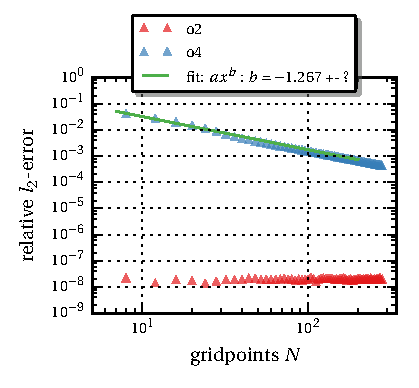
\includegraphics{gfx/immersed_boundary/poiseuille_flow/3_df/relative_l2error.pdf}
    \caption{Relative $l_2$-error for the DF-FD2 and DF-FD4 method.}
    \label{fig:vali_pflow_3gc}
\end{figure}

\begin{figure}[!h]
  \centering
  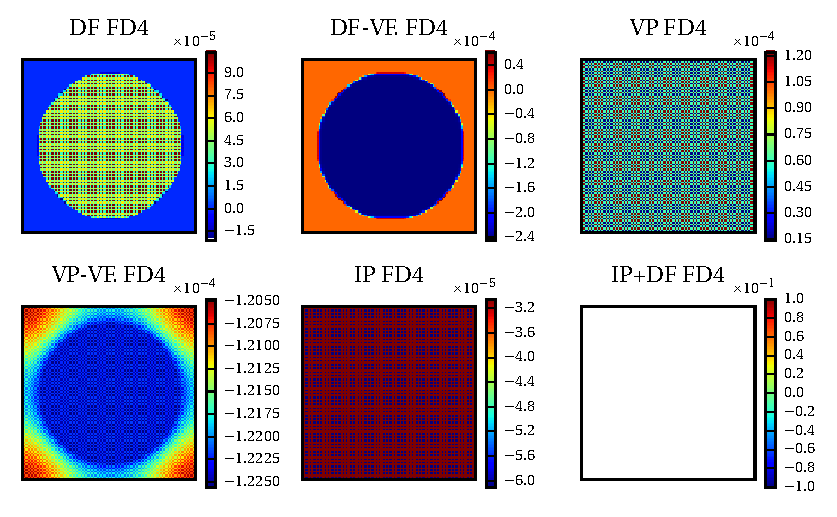
\includegraphics{gfx/immersed_boundary/hpflow/long/rho.pdf}
  \caption{Densitiy oscillations for different immersed boundary methods with the use  of 4th order finite difference schemes.}
    \label{fig:hpflow_allgc_theo}
\end{figure}

\chapter{Source Code}

%\begin{lstlisting}[caption='RK-Stability Computation']
\section{Runge-Kutta stability computation}
\begin{python}
import matplotlib.pyplot as plt
import numpy as np
from math import factorial as fac
from scipy import interpolate

def radial_sort(x, y):
    """Sort line by angle from center (-1, 0)"""
    angle = np.arctan2(y, x + 1.)
    idx = angle.argsort()
    x, y = x[idx], y[idx]
    # Split at opening in line
    dx = np.diff(np.append(x, x[-1]))
    dy = np.diff(np.append(y, y[-1]))
    max_gap = np.abs(np.hypot(dx, dy)).argmax() + 1
    x = np.append(x[max_gap:], x[:max_gap])
    y = np.append(y[max_gap:], y[:max_gap])
    return x, y

def main():
    f, ax = style.newfig(0.8)
    x = np.linspace(-4, 4, 1500)
    X, Y = np.meshgrid(x, x)
    C = X + 1j*Y

    for i in range(1,6)[::-1]:
        b = np.zeros_like(C)
        for j in range(0,i):
            b += C**j/fac(j)
        out = np.where(np.diff((np.abs(b)<=1).astype('float')) != 0)
        pts = np.column_stack((X[out], Y[out]))
        x, y = pts[:, 0], pts[:, 1]
        try:
            x, y = radial_sort_line(x,y)
            x = np.append(x, x[0])
            y = np.append(y, y[0])

            tck, u = interpolate.splprep([x, y], s=0)
            unew = np.linspace(0, 1.0, 100)
            out = interpolate.splev(unew, tck)
            plt.plot(out[1], out[0])
        except:
            print 'Error for %i' % i
    plt.show()

if __name__=='__main__':
    main()

\end{python}
%#\end{lstlisting}
\clearpage

\section{Chapter 1}
The contents...
\chapter{Python API}
Addional Figures and Calculations
